\documentclass[10pt,onecolumn]{article}
\usepackage[utf8]{inputenc}
 
\pagenumbering{arabic}
\usepackage{siunitx}
\usepackage{graphicx}
\usepackage{float}
\usepackage{placeins}
\usepackage{adjustbox}
\usepackage[ruled,vlined,linesnumbered]{algorithm2e}
\usepackage{tablefootnote}
\usepackage{mathtools}
\usepackage[margin=0.75in]{geometry} %This is for all the margins

\def\@maketitle{%
  \null
  \vskip 2em%
  \begin{center}%
  \let \footnote \thanks
    {\LARGE \@title \par}%
    \vskip 1.5em%
    {\large
      \lineskip .5em%
      \begin{tabular}[t]{c}% <------
        \@author%            <------ Authors
      \end{tabular}\par}%    <------
    \vskip 1em%
  %  {\large \@date}%
  \end{center}%
  \par
  \vskip 1.5em}

\date{25/02/2019}

\title{\vspace{-2.2cm} \textbf{ELEN4020: Data Intensive Computing \\ Laboratory Exercise 1}}
\author{\begin{tabular}{ll}
  Lynch Mwaniki & 1043475 \\
  Madimetja Sethosa & 1076467 \\
  Teboho Matsheke & 1157717 \\
\end{tabular}
 }


\begin{document}
%\centering
\title{\Large{\textbf{ ELEN4020: Data Intensive Computing \\ }}}

\maketitle
\thispagestyle{empty}\pagestyle{empty}
\vspace{-8mm}

\section*{Multi-Dimensional Arrays}
A common way to access elements in multidimensional arrays requires iterating through the dimensions using nested loops. The number of loops required is directly proportional to the number of dimensions of the array. This method allows elements to be accessed in a static array, but it is computationally expensive. This method would be difficult to implement when working with dynamic arrays and would also increase computation time.\\

\noindent In computer memory, arrays are stored as a contiguously. In the C programming language, arrays are stored in memory using row major order. The co-ordinates of the elements in an N dimensional array can be transformed to a 1-dimensional co-ordinate system. This allows for easy access to the elements by using a pointer, thus eliminating the need for nested loops.

\section*{3D Matrix Multiplication}
In order to simplify the 3D matrix multiplication an expansion is made on the 2d matrix multiplication concept. The 3D matrices are represented as layers of 2d matrices. If a 3D matrix A is of size (N,N,N), it will consist of N 2d matrices with sizes (N,N).
\subsection*{rank3TensorMult function}
\noindent The function takes two pointers to the two 3D matrices being multiplied, their \textit{size} and \textit{total number of elements}. It is assumed that the two matrices being multiplied are of the same size, thus there is no size checking function. Firstly, an array is created using the \textit{total number of elements} to store the multiplication results. A \textbf{for} loop is used to traverse through the two 3D matrices to extract the \textit{N} 2D layers. In each loop, the 2D layers are fed to the \textit{rank2TensorMult()} function and the results are then pushed into the results array. The representation can be viewed from Figure \ref{fig:3Dmult}.

\begin{figure}[H]
\centering
  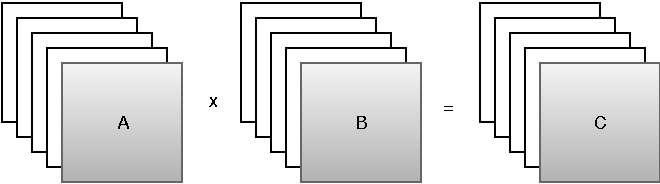
\includegraphics[width=5in]{3Dmult.pdf}
  \caption{3D matrix layer multiplication.}
  \label{fig:3Dmult}
\end{figure}

\noindent The \textit{rank2TensorMult()} function uses one \textbf{for} loop to do the computations, this results in a total of two \textbf{for} loops for the \textit{rank3TensorMult()} function. For more details about the function and other assisting functions, see Appendix A for the Pseudo code. 


\clearpage
\appendix
\label{App:Apendix}
\section{Pseudo code}
\subsection{allocateMatrix}
    \begin{algorithm}[H]
        \caption{Allocate Matrix in Memory}
        \KwResult{Integer pointer, pointing to first element of matrix.}
        \SetKwInOut{Input}{Input}\SetKwInOut{Output}{Output}
        \Input{Total Number of Elements}
        result\_ptr = (int*)calloc(number\_of\_elements, sizeof(int)) \\
        \Return result\_ptr
    \end{algorithm}

\subsection{getElementLocation2D}
    \begin{algorithm}[H]
        \caption{Get Location of Element in 2D matrix when represented as 1D Array}
        \KwResult{Integer containing position of element in 1D matrix}
        \SetKwInOut{Input}{Input}\SetKwInOut{Output}{Output}
        \Input{1D Array containing indexes}
        \Input{Dimension N}
        row = index[0]\\
        column = index[1]\\
        \Return $(row*N)+column$
    \end{algorithm}
  

\subsection{retrieveElement2D}
    \begin{algorithm}[H]
        \caption{Retrieve Element from 2D matrix}
        \KwResult{Integer value of the element in the 2D matrix co-ordinates.}
        \SetKwInOut{Input}{Input}\SetKwInOut{Output}{Output}
        \Input{Pointer to matrix, 1D Array containing indexes}
        \Input{Dimension N}
        \Return $*(matrix\_ptr + getElementLocation2D(indexes, N))$
    \end{algorithm}
    
\subsection{rank2TensorMult}
    \begin{algorithm}[H]
        \caption{2D Matrix Multiplication Algorithm}
        \KwResult{Integer pointer, pointing to first element of product matrix.}
        \SetKwInOut{Input}{Input}\SetKwInOut{Output}{Output}
        \Input{Pointer to matrix A, Pointer to matrix B}
        \Input{Matrix dimensions (N), Total number of elements in matrix}
        
        result\_ptr = allocateMatrix(number\_of\_elements) \\
        total\_multiply\_operations = $number\_of\_elements \cdot N$ \\
        \For{m=0 to total\_multiply\_operations-1}
        { i = $ m \div number\_of\_elements $ \\
          j = m mod N \\
          k = $ (m \div N)$ mod N \\
          
          indexA = [i, k] \\
          indexB = [k, j] \\
          
          elementA = retrieveElement2D(matrixA, indexA, N)\\
          elementB = retrieveElement2D(matrixB, indexB, N)\\
          
          indexC = [i, j]\\
          total\_ptr = result\_ptr + getElmentLocation2D(indexC, N) \\
          *total\_ptr = *total\_ptr + $(elementA \cdot elementB)$
        }%for
        \Return result\_ptr
    \end{algorithm}
    
    \subsection{rank3TensorMult}
    \begin{algorithm}[H]
        \caption{3D Matrix Multiplication Algorithm}
        \KwResult{Integer pointer, pointing to first element of product matrix.}
        \SetKwInOut{Input}{Input}\SetKwInOut{Output}{Output}
        \Input{Pointer to matrix A, Pointer to matrix B}
        \Input{Matrix dimensions (N), Total number of elements in matrix}
        results3D = allocateMatrix(number\_of\_elements)
        startPos = 0\\
        elements2D = N*N\\
        \For{m=0 to N}
        { 
            results2D = rank2TensorMult(matrix A+startPos, matrix B+startPos, N, elements2D)
        
            \For{i=0 to elements2D}
            {
                results3D = results2D\\
                results2D++;\\
                results3D++;
                
            }
            startPos += elements2D;\\
            results2D = results2D - elements2D;
        }%for
        \Return result3D 
    \end{algorithm}
\end{document}